\begin{comment}
\end{comment}

\begin{center}
\thispagestyle{empty}
%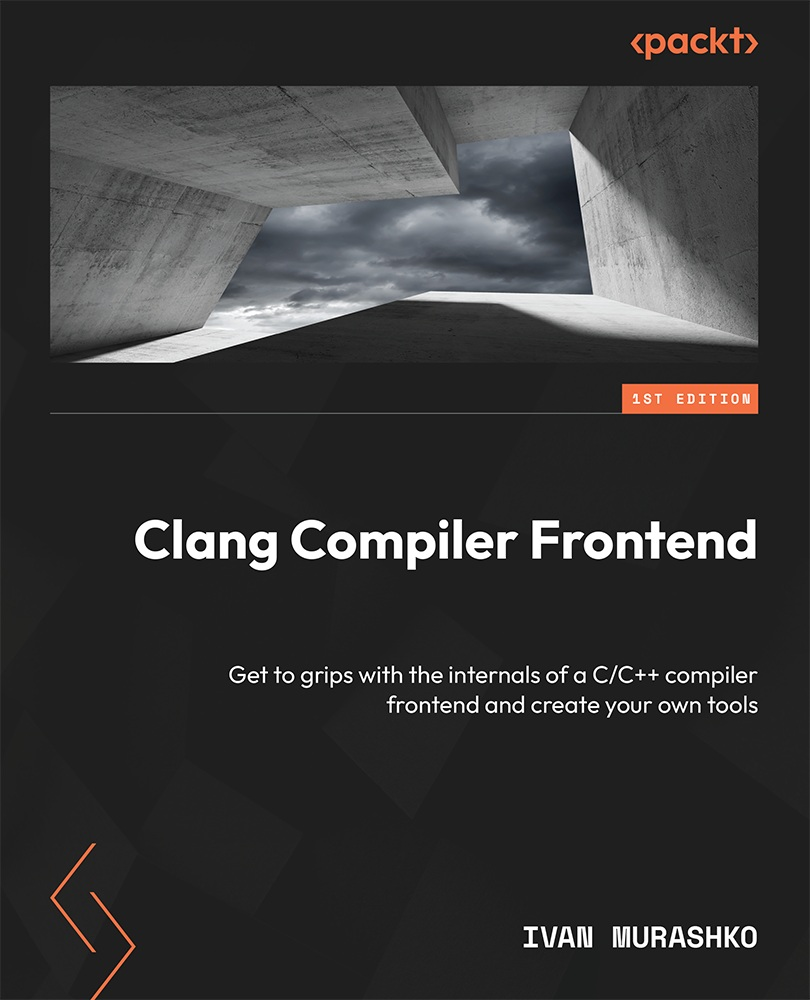
\includegraphics[width=\textwidth,height=\textheight,keepaspectratio]{cover.png}
\begin{tikzpicture}[remember picture, overlay, inner sep=0pt]
\node at (current page.center)
{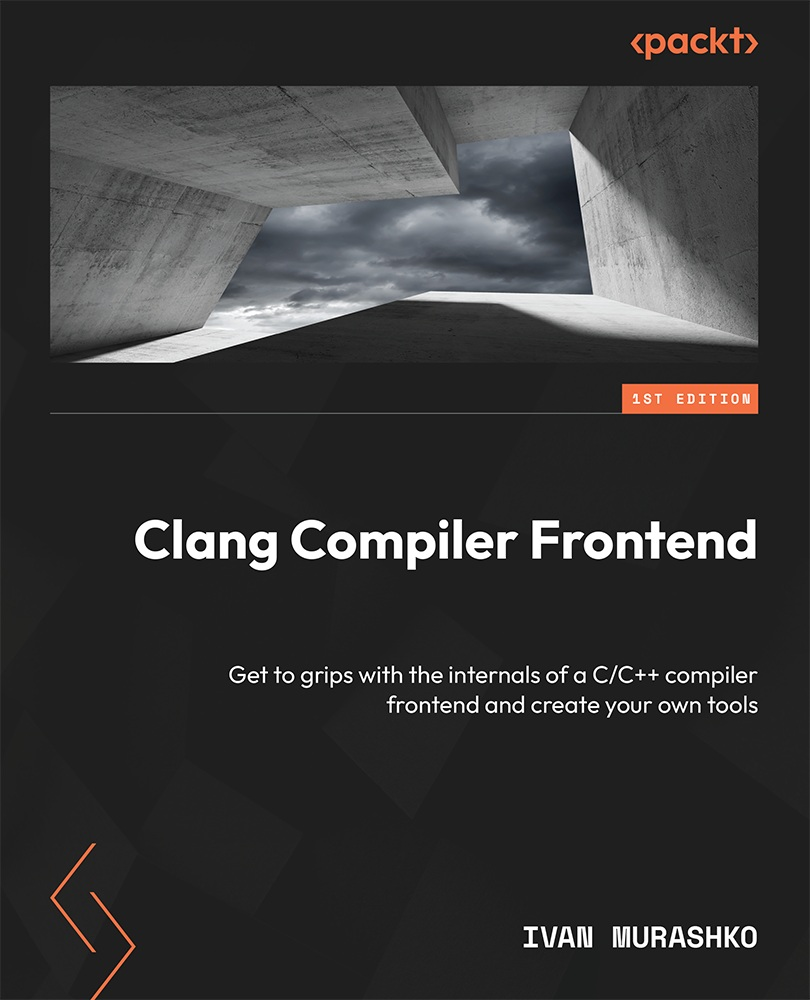
\includegraphics[width=\paperwidth, keepaspectratio=false]{cover.png}};
\end{tikzpicture}
\newpage
\thispagestyle{empty}
\huge
\textbf{Clang Compiler Frontend}
\\[9pt]
{\Large 掌握 C/C++ 编译器前端的工作原理并创建自己的工具。}
\\[9pt]
\normalsize
作者: Ivan Murashko
\\[8pt]
\normalsize
译者:\href{https://github.com/xiaoweiChen/Clang-Compiler-Frontend}{陈晓伟}
\\[8pt]
\end{center}

\newpage

\pagestyle{empty}
\tableofcontents
\newpage


\setsecnumdepth{section}

\myPart{}{关于作者}{about-the-author.tex}
\newpage

\myPart{}{关于评审}{about-the-reviewer.tex}
\newpage

\myPart{}{前言}{preface.tex}
\newpage

\myPart{第一部分}{Clang的安装和架构}{part1/title.tex}
\newpage

\myChapter{第1章}{环境配置}{part1/chapter1/0.tex}
\mySubsection{1.1.}{主要内容}{part1/chapter1/1.tex}
\mySubsection{1.2.}{了解LLVM}{part1/chapter1/2.tex}
\mySubsection{1.3.}{编译源码}{part1/chapter1/3.tex}
\mySubsection{1.4.}{测试项目——使用Clang工具进行语法检查}{part1/chapter1/4.tex}
\mySubsection{1.5.}{总结}{part1/chapter1/5.tex}
\mySubsection{1.6.}{扩展阅读}{part1/chapter1/6.tex}
\newpage

\myChapter{第2章}{Clang的架构}{part1/chapter2/0.tex}
\mySubsection{2.1.}{源码位置}{part1/chapter2/1.tex}
\mySubsection{2.2.}{开始使用编译器}{part1/chapter2/2.tex}
\mySubsection{2.3.}{Clang驱动概述}{part1/chapter2/3.tex}
\mySubsection{2.4.}{Clang前端概述}{part1/chapter2/4.tex}
\mySubsection{2.5.}{总结}{part1/chapter2/5.tex}
\mySubsection{2.6.}{扩展阅读}{part1/chapter2/6.tex}
\newpage

\myChapter{第3章}{Clang AST}{part1/chapter3/0.tex}
\mySubsection{3.1.}{源码位置}{part1/chapter3/1.tex}
\mySubsection{3.2.}{AST}{part1/chapter3/2.tex}
\mySubsection{3.3.}{遍历AST}{part1/chapter3/3.tex}
\mySubsection{3.4.}{递归AST访问器}{part1/chapter3/4.tex}
\mySubsection{3.5.}{AST匹配器}{part1/chapter3/5.tex}
\mySubsection{3.6.}{使用clang-query探索Clang AST}{part1/chapter3/6.tex}
\mySubsection{3.7.}{处理AST的错误}{part1/chapter3/7.tex}
\mySubsection{3.8.}{总结}{part1/chapter3/8.tex}
\mySubsection{3.9.}{扩展阅读}{part1/chapter3/9.tex}
\newpage

\myChapter{第4章}{基本库和工具}{part1/chapter4/0.tex}
\mySubsection{4.1.}{源码位置}{part1/chapter4/1.tex}
\mySubsection{4.2.}{LLVM编码风格}{part1/chapter4/2.tex}
\mySubsection{4.3.}{LLVM基本库}{part1/chapter4/3.tex}
\mySubsection{4.4.}{Clang基本库}{part1/chapter4/4.tex}
\mySubsection{4.5.}{LLVM支持工具}{part1/chapter4/5.tex}
\mySubsection{4.6.}{Clang插件项目}{part1/chapter4/6.tex}
\mySubsection{4.7.}{总结}{part1/chapter4/7.tex}
\mySubsection{4.8.}{扩展阅读}{part1/chapter4/8.tex}
\newpage

\myPart{第二部分}{Clang工具}{part2/title.tex}
\newpage

\myChapter{第5章}{Clang-Tidy代码检查框架}{part2/chapter5/0.tex}
\mySubsection{5.1.}{源码位置}{part2/chapter5/1.tex}
\mySubsection{5.2.}{Clang-Tidy概述和使用示例}{part2/chapter5/2.tex}
\mySubsection{5.3.}{Clang-Tidy的内部设计}{part2/chapter5/3.tex}
\mySubsection{5.4.}{自定义Clang-Tidy检查}{part2/chapter5/4.tex}
\mySubsection{5.5.}{总结}{part2/chapter5/5.tex}
\mySubsection{5.6.}{扩展阅读}{part2/chapter5/6.tex}
\newpage

\myChapter{第6章}{高级代码分析}{part2/chapter6/0.tex}
\mySubsection{6.1.}{源码位置}{part2/chapter6/1.tex}
\mySubsection{6.2.}{静态分析}{part2/chapter6/2.tex}
\mySubsection{6.3.}{CFG}{part2/chapter6/3.tex}
\mySubsection{6.4.}{自定义CFG检查}{part2/chapter6/4.tex}
\mySubsection{6.5.}{Clang中的CFG}{part2/chapter6/5.tex}
\mySubsection{6.6.}{Clang分析工具的简要描述}{part2/chapter6/6.tex}
\mySubsection{6.7.}{分析的局限性}{part2/chapter6/7.tex}
\mySubsection{6.8.}{总结}{part2/chapter6/8.tex}
\mySubsection{6.9.}{扩展阅读}{part2/chapter6/9.tex}
\newpage

\myChapter{第7章}{重构工具}{part2/chapter7/0.tex}
\mySubsection{7.1.}{源码位置}{part2/chapter7/1.tex}
\mySubsection{7.2.}{自定义代码修改工具}{part2/chapter7/2.tex}
\mySubsection{7.3.}{Clang-Tidy——代码修改工具}{part2/chapter7/3.tex}
\mySubsection{7.4.}{修改代码和Clang-Format}{part2/chapter7/4.tex}
\mySubsection{7.5.}{总结}{part2/chapter7/5.tex}
\mySubsection{7.6.}{扩展阅读}{part2/chapter7/6.tex}
\newpage

\myChapter{第8章}{集成开发环境支持与 Clangd}{part2/chapter8/0.tex}
\mySubsection{8.1.}{源码位置}{part2/chapter8/1.tex}
\mySubsection{8.2.}{语言服务器协议}{part2/chapter8/2.tex}
\mySubsection{8.3.}{环境设置}{part2/chapter8/3.tex}
\mySubsection{8.4.}{LSP示例}{part2/chapter8/4.tex}
\mySubsection{8.5.}{集成Clang工具}{part2/chapter8/5.tex}
\mySubsection{8.6.}{性能优化}{part2/chapter8/6.tex}
\mySubsection{8.7.}{总结}{part2/chapter8/7.tex}
\mySubsection{8.8.}{扩展阅读}{part2/chapter8/8.tex}
\newpage

\myPart{第三部分}{附录}{part3/title.tex}
\newpage

\myChapter{附录A}{编译数据库}{part3/appendix-A/0.tex}
\mySubsection{A.1.}{定义}{part3/appendix-A/1.tex}
\mySubsection{A.2.}{创建CDB}{part3/appendix-A/2.tex}
\mySubsection{A.3.}{Clang工具和CDB}{part3/appendix-A/3.tex}
\mySubsection{A.4.}{扩展阅读}{part3/appendix-A/4.tex}
\newpage

\myChapter{附录B}{优化构建速度}{part3/appendix-B/0.tex}
\mySubsection{B.1.}{源码位置}{part3/appendix-B/1.tex}
\mySubsection{B.2.}{预编译头文件}{part3/appendix-B/2.tex}
\mySubsection{B.3.}{Clang模块}{part3/appendix-B/3.tex}
\mySubsection{B.4.}{扩展阅读}{part3/appendix-B/4.tex}
\newpage
